\documentclass{article}
\usepackage{xeCJK}
\usepackage{amsmath}
\usepackage{graphicx}

\setCJKmainfont{Microsoft YaHei}
\linespread{1.5}
\setlength{\parindent}{0pt}

\begin{document}
1. \\
\[
\begin{aligned}
    & G = (\{S, A, B\}, \{a, b, c, d\}, P, S) \\
    & P: A \rightarrow \varepsilon | aAb,\quad B \rightarrow \varepsilon | cBd, \quad S \rightarrow AB    
\end{aligned}
\]

2. \\
\[
\begin{aligned}
    & G = (\{S, A\}, \{a, b\}, P, S) \\
    & P: A \rightarrow \varepsilon | aAb,\quad S \rightarrow a^2A
\end{aligned}    
\]

(3) \\
q0 是起始状态,q0、q1 是接受状态。\\
PDA 如下图所示:
\begin{figure}[htbp]
	\centering
    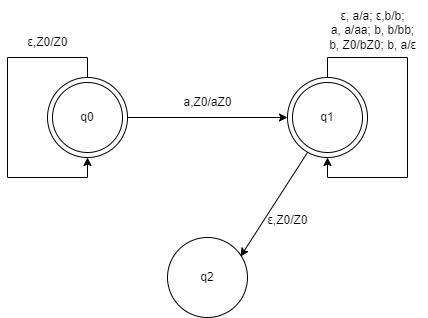
\includegraphics[width=20em,height=!]{PDA.png}
	\caption{$PDA$}
\end{figure}

4.\\
(1)\\
\[
\begin{aligned}
    & G_1 = (\{S, A, B\}, \{a, b, c\}, P_1, S) \\
    & P_1: A \rightarrow \varepsilon | aBb^2, \quad b \rightarrow \varepsilon | Bc, \quad S \rightarrow AB \\
    \\
    & G_2 = (\{S, A, B\}, \{a, b, c\}, P_2, S) \\
    & P_2: A \rightarrow \varepsilon | Aa, \quad B \rightarrow \varepsilon | bBc^3,\quad S \rightarrow AB
\end{aligned}    
\]
(2)\\
$L_1 \cap L_2$ 不是 CFG。 \\
证明:\\
记 $L = L_1 \cap L_2 = \{a^nb^{2n}c^{6n},\; n \geq 0\}$, \\
假设 $L$ 是 CFG,则存在正整数 $N$,对 $\forall z \in L (|z| \geq N)$ 满足泵引理。 \\
从 $L$ 中取 $z = a^Nb^{2N}c^{6N}$,显然 $z \in L$ 且 $|z| = 9N \geq N$。 \\
由泵引理,$z$ 可被分为 $z = uvwxy$,且有 $|vwx| \leq N$,$|vx| \neq \varepsilon$,\\
那么 $vx$ 可能为:\\
i.只包含 a 或 b 或 c; \\
ii.只包含 a 和 b, 或 只包含 b 和 c; \\
对这两种情况,$uv^0wx^0y \notin L$;\\
所以假设不成立, $L$ 不是 CFG。\\
\end{document}

